% !TEX encoding = UTF-8 Unicode

\documentclass[a4paper]{article}

\usepackage{color}
\usepackage{url}
%\usepackage[T2A]{fontenc} % enable Cyrillic fonts
\usepackage[T1]{fontenc} % enables proper hyphenation of words with characters š đ č ć ž
\usepackage[utf8]{inputenc} % make weird characters work
\usepackage{graphicx}
\usepackage{listings}
\usepackage{pdfpages}

\usepackage{caption}
\usepackage{subcaption}

\usepackage[english,serbian]{babel}
\usepackage[unicode]{hyperref}
\hypersetup{colorlinks,citecolor=green,filecolor=green,linkcolor=blue,urlcolor=blue}


\begin{document}
%Relevant Images in HTML
\title{Relevantne slike u HTML-u\\ \small{Seminarski rad u okviru kursa\\Mašinsko učenje\\ Matematički fakultet}}

\author{Mirko Brkušanin\\ mirkobrkusanin94@gmail.com}
\date{septembar 2018.}
\maketitle

\abstract{
Veb stranice članaka na internetu mogu sadržati veliki broj slika. Ljudima nije teško prepoznati koje slike su relevantne za taj članak a koje predstavljaju linkove ka drugim člancima, reklamama ili su samo ukrasni elementi. Međutim razviti model koji može sa velikom preciznošću da odlučuje o tipu slike nije lak posao. Uzimajući samo HTML kod nekog članka i bez samih slika prikazujemo način obučavanja modela koji može da razlikuje ove dve klase slika.

Ovaj rad predstavlja proveru ideje i nadogradnju postupka predstavljenog u: ,,Relevanseek: Determining relevant images from HTML source'' David Zhang, 2013. \cite{relevanseek}
}

\tableofcontents

\newpage

\section{Uvod}
\label{sec:uvod}

U početku veb stranice su se sastojale samo od teksta. Ubrzo je ostvarena mogućnost ugrađivanja slika unutar stranica. Danas kada imamo značajno veće protoke podataka imamo i veb stranice koje mogu biti pune raznog multimedijalnog sadržaja. 
	
Kada su u pitanju razni članci na iternetu, pored samog sadržaja o temi o kojoj se govori kao i pratećih slika često imamo i veći broj sporednih slika koje mogu predstavljati linkove ka drugim člancima ili mogu biti reklame. Takođe mogu biti i dugmići koje nude mogućnost deljenja sadržaja na društvenim mrežama ili mogu biti samo ukrasni elementi poput logo-a. Dok ljudima nije problem razaznati između slika koje pripadaju članku od sporednih, automatizacija tog postupka nije laka. 
	
Kompanija Diffbot\cite{diffbot} koja razvija razne resurse koji pomažu prilikom izvlačenja podataka iz veb stranica je 2013. godine postavila izazov u kojem je trebalo na osnovu HTML dokumenta nekog članka odrediti koje su slike relevantne. Rešenje koje je pobedilo je opisano u radu: \textit{,,Relevanseek: Determining relevant images from HTML source'', David Zhang, 2013.}\cite{relevanseek}. U ovom radu će biti izvršena provera ideje i nadogradnje spomenutog rada.
	
Prvo će biti obavljen pregled ponuđenih podataka na kojima treba trenirati model. Zatim kako i koje su bitne informacije o slikama sakupljene, a potom rezultati obučavanja prikladnih modela. 
	
\section{Skup podataka}
\label{sec:podaci}

Diffbot je ponudio oko 600 stranica koje predstavljaju skup za treniranje. Svaki stranica je predstavljena samo sa HTML datotekom iz koje su ukolonjeni svi skriptovi. Takođe ne postoje ni prateći CSS dokumenti. Otvaranjem dokumenata u internet pregledaču ne možemo dobiti tačan prikaz elemenata kao ni njihov raspored ili pozicije. Međutim, Diffbot je uneo dodatne podatke u određene HTML tag-ove koji pružaju informaciju o načinu prikaza. U pitanju je atribut ,,\_'' koji može izgledati ovako:
	
\begin{lstlisting}
<img src="..." alt="..." _="x=125,y=742,w=160,h=160,
dis=block,bre=repeat,fsi=11px,ffa=Arial;sans-serif,
tal=left,co=61;61;61;255,lhe=13px,lst=disc">
\end{lstlisting}

Neke od značajnih informacija koje možemo saznati su pozicija kao i veličina prikaza određenog HTML elementa.

Zajedno sa HTML dokumentima dolazi i jedna JSON datoteka koja opisuje koje slike su zapravo relevantne za koji dokument. Releventne slike su date kao string koji predstavlja XPath izraz i označava putanju do odgovarajućih elemenata u HTML stablu.

\begin{lstlisting}
"/html/body/div[3]/div/div/div[4]/div[5]/div[3]/img"
\end{lstlisting}

\subsection{Prljavi podaci}
Spomenuta JSON datoteka sa oznakama relevantnih slika sadrži u sebi više grešaka. One se odnose upravo na XPath izraz koji ne pokazuje uvek na pravu sliku. Kako je ispravnost ulaznih podataka od ključnog značaja za pravilno obučavanje modela, neke očigledne greške su ručno ispravljene pre obrade podataka. Najčešći slučaj nepravilnosti koji je bio uočen je nepostojanje makar jedne slike u dokumentu koja je označena kao relevantna. Kako je \textit{url} originalnog članka dat zajedno sa datotekom, često se može uočiti da postoje slike koje ispunjavaju ove kriterijume. Od 598 unosa u datoteci sa oznakama napravljene su korekcije za 24 dokumenta. Sve korekcije su donete na osnovu ručnog suđenja autora \footnote{Lista izmena je dokumentovana u datoteci \textit{corrections.txt} koja se može pornaći zajedno sa kodom projekta. Kako je svaka provera vršena ručnim pregledom koda, ispravljane su samo očigledne greške. Provera ostalih dokumenata nije izvršena. U nekim slučajevima \textit{url} originalnog članka nije bio dostupan ili se znatno razlikovao zbog čega se ne garantuje da su izmene uvek korektne.}.  

\section{Atributi}
\label{sec:atributi}

Pre nego što počnemo sa treniranjem bilo kog modela prvo moramo pravilno izvući atribute iz HTML dokumenata. Prirodno se postavlja pitanje na osnovu kojih atributa neke slike možemo zaključiti da li je ona relevantna. 

Projekat je u potpunosti napisan u Python jeziku, pa je za parsiranje i izvlačenje atributa iz dokumenata korišćena biblioteka \textit{Beautiful Soup 4} \cite{bs4}. Ona nam pomaže da od HTML dokumenta napravimo stablo čiji su čvorovi HTML tagovi, a zatim pomoću drugih funkcija iz biblioteke možemo lako da pronađemo odgovarajuće elemente kao i njihova svojstva. \\
Neki od atributa koji su izvučeni iz dokumenata su:
\begin{itemize}
	\item x i y koordinata prikaza slika kao i dimenzije slike
	\item vrednosti \textbf{src}, \textbf{alt} i \textbf{title} atributa slike ukoliko postoje
	\item da li je slika hiperlink
	\item dimenzije najmanjeg pretka koji se prikazuje
	\item da li se u atributima \textbf{class} ili \textbf{id} elementa slike ili nekog njenog pretka nalazi neki karakterističan string
	\item rastojanje od ivica dokumenta
\end{itemize}
Neki atributi kao što je \textbf{src} sami po sebi ne predstavljaju korisnu informaciju jer ih ne možemo prevesti u numeričku vrednost. Međutim, možemo ih iskoristiti za izvođenje novih atributa. Neki od tih atributa su:
%Nakon određivanja vrednosti ovih atributa iz njih dalje možemo izvesti nove:
\begin{itemize}
	\item da li je slika lokalni ili eksterni resurs (na osnovu \textbf{src} atributa)
	\item edit rastojanje \textbf{src}, \textbf{alt} i \textbf{title} atributa slike od \textbf{title} atributa dokumenta
	\item broj slika sa istim dimenzijama u dokumentu
	\item da li je slika nacrtana unutar granica dokumenta
\end{itemize}
Neke vrednosti unutar jednog dokumenta se ne mogu uvek porediti sa vrednosti drugog dokumenta. Npr. spomenuto edit rastojanje nekih atributa u odnosu sa naslovom dokumenta će imati veće vrednosti za svaku sliku u dokumentu samim tim što je niska naslova duža. Prema tome neke atribute treba posmatrati samo u odnosu sa drugim slikama u istom dokumentu. Sledeći atributi dobijeni su normalizacijom ili standardizacijom vrednosti pojedinačno za svaki dokument:
\begin{itemize}
	\item standardizovana edit rastojanja \textbf{src}, \textbf{alt} i \textbf{title} atributa slike od \textbf{title} atributa dokumenta
	\item relativne koordinata i dimenzije slika
	\item relativna rastojanja slike od ivica
	\item relativne dimenzije najmanjeg pretka
\end{itemize}
Sveukupno imamo 48 atributa. Kada uklonimo atribute koji su samo korišćeni za izvođenje drugih i one koji nisu numeričke vrednosti ostane nam 28 atributa ne računajući ciljni atribut.

Ciljni atribut određujemo na osnovu XPath izraza koje je dat za svaki dokument. Nažalost, \textit{Beautiful Soup 4} ne sadrži mogućnost pronalaženja elemenata na ovaj način pa je korišćena biblioteka \textit{lxml} \cite{lxml}.

\section{Rezultati klasifikacije}

U datom skupu za treniranje od 600 dokumenata nalazi se 29835 slika od kojih su samo 935 relevantne slike. Broj nerelevantnih slika je veći od 96\%. Zbog toga koristimo F1 meru kao ocenu kvaliteta modela umesto tačnosti klasifikacije (\emph{engl. accuracy}).

Kao najpouzdaniji metod se pokazao metod potpornih vektora (\emph{engl. SVM}). Za testiranje je korišćena biblioteka \textit{sklearn} \cite{sklearn}. Rezultati testiranja klasifikatora SVC nad skupom podataka za različite kernele se mogu videti na slici \ref{fig:svc-results}.

%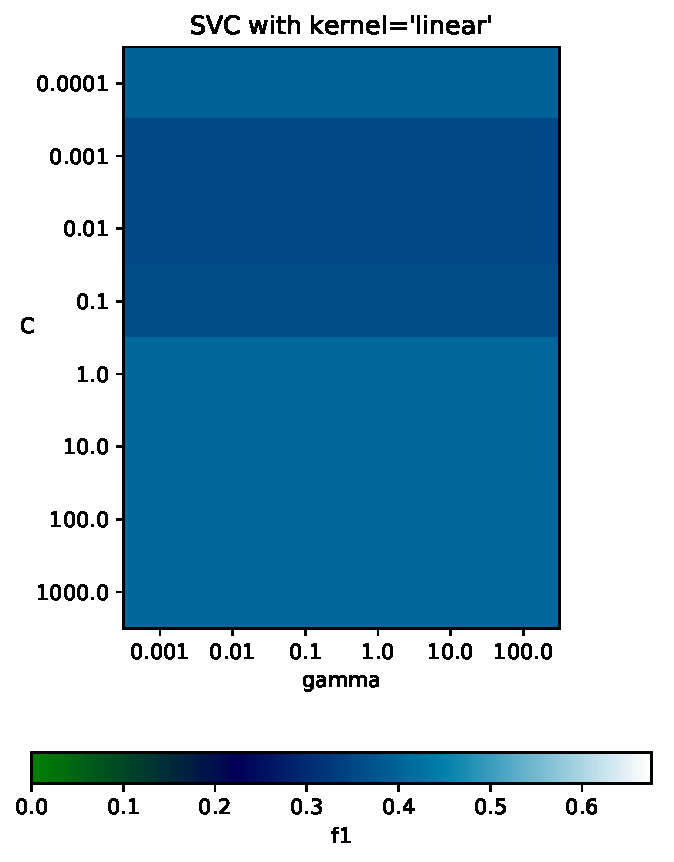
\includepdf[]{images/SVC_kernel_linear.pdf}
%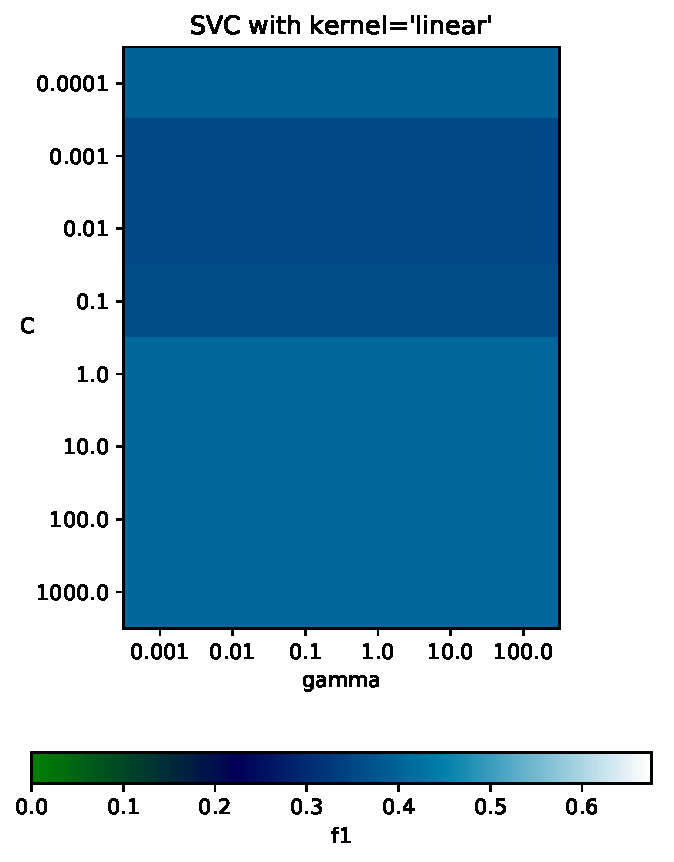
\includegraphics[]{images/SVC_kernel_linear.pdf}

\begin{figure}
	\centering
	\begin{subfigure}{.5\textwidth}
		\centering
		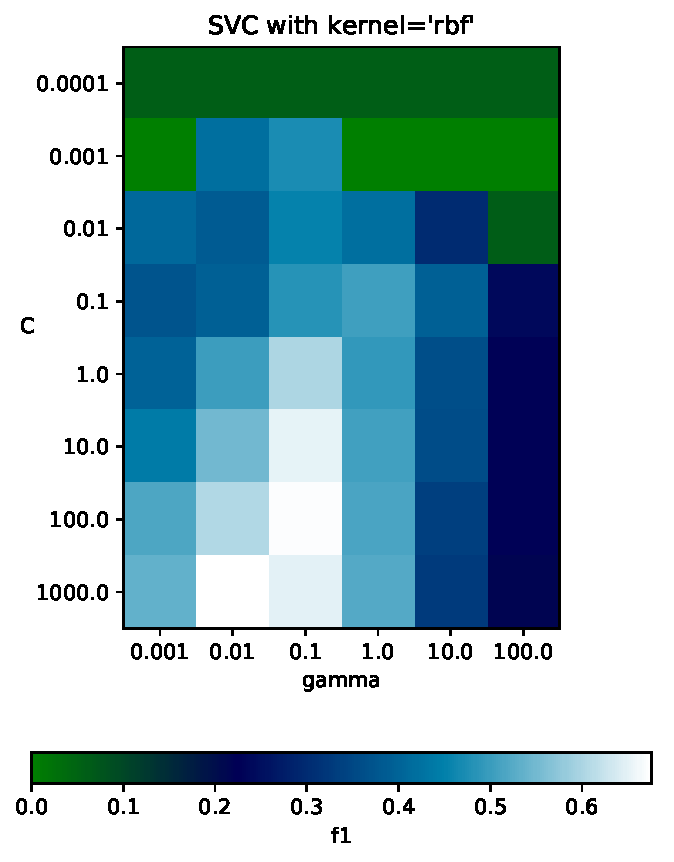
\includegraphics[width=.8\linewidth]{images/SVC_kernel_rbf.pdf}
		\caption{Rezultati za rbf kernel \hfill \break \hfill \break \hfill \break}
		\label{fig:sub1}
	\end{subfigure}% \hfill% or \hspace{5mm} or \hspace{0.3\textwidth}
	\begin{subfigure}{.5\textwidth}
		\centering
		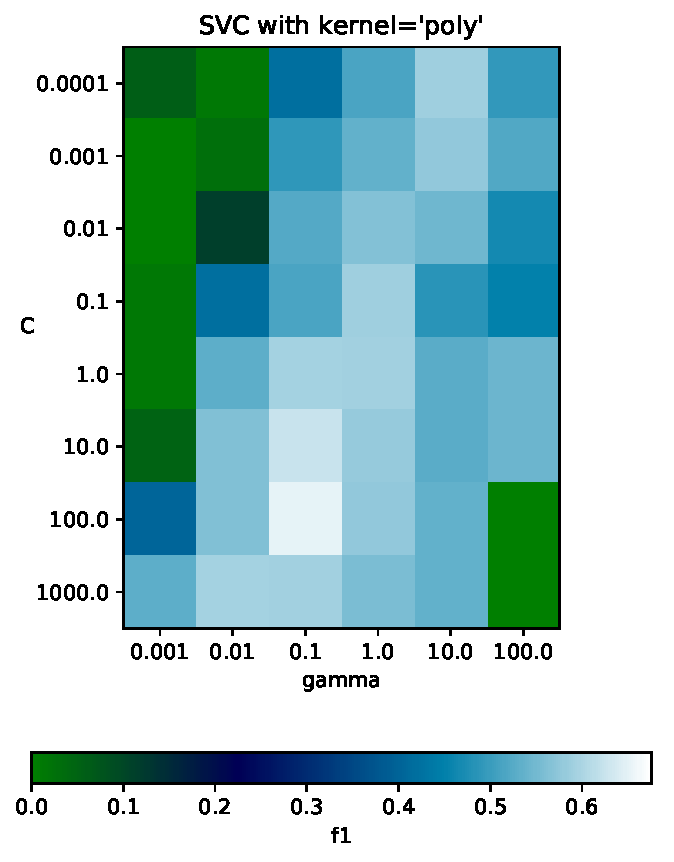
\includegraphics[width=.8\linewidth]{images/SVC_kernel_poly.pdf}
		\caption{Rezultati za polinomijanlni kernel (vrednosti za gamma=100 nisu izračunate za C>10 zbog dugog vremena obučavanja modela)}
		\label{fig:sub2}
	\end{subfigure}
	\begin{subfigure}{.5\textwidth}
		\centering
		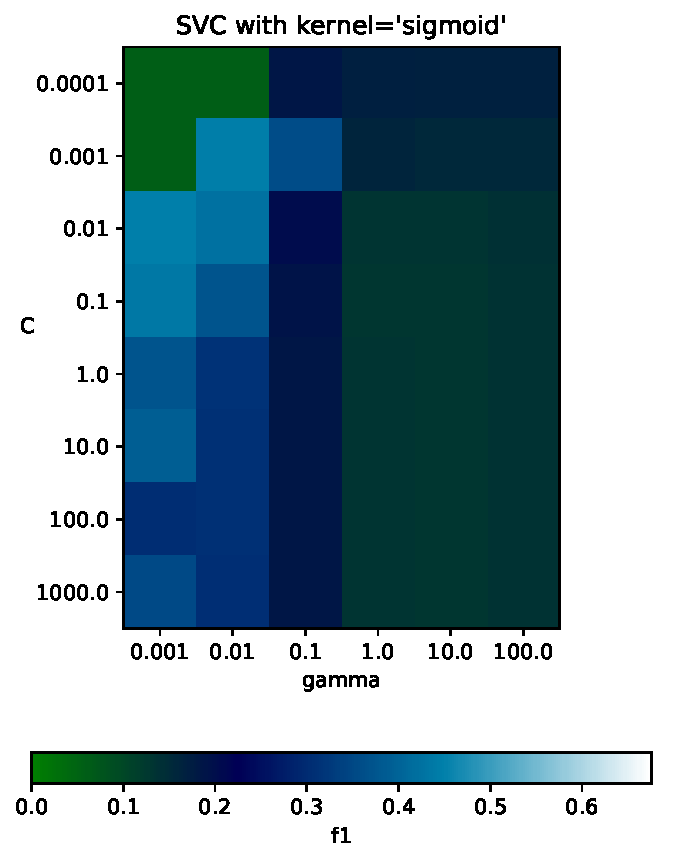
\includegraphics[width=.8\linewidth]{images/SVC_kernel_sigmoid.pdf}
		\caption{Rezultati za sigmoidni kernel \hfill \break\hfill \break\hfill \break}
		\label{fig:sub3}
	\end{subfigure}%
	\begin{subfigure}{.5\textwidth}
		\centering
		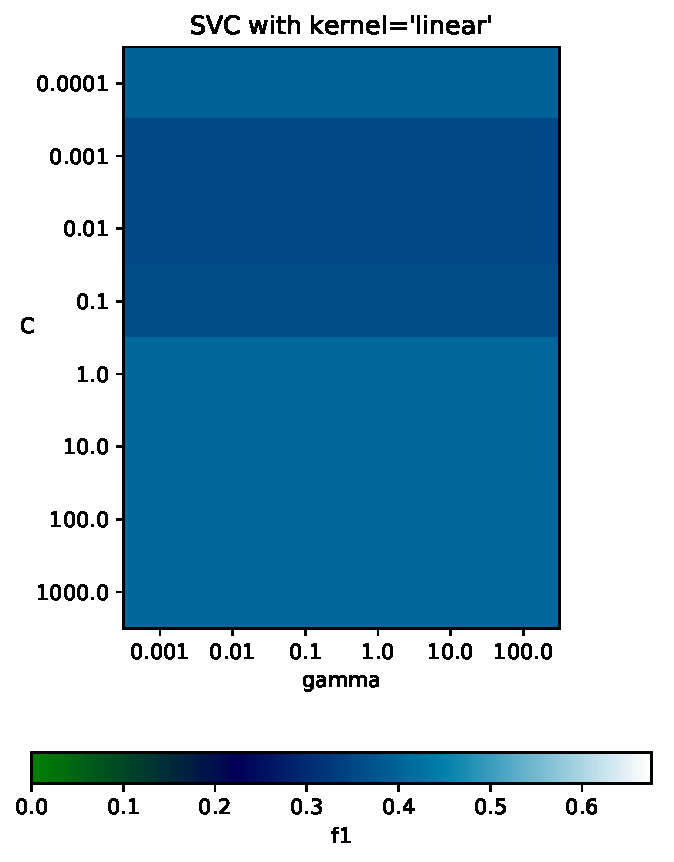
\includegraphics[width=.8\linewidth]{images/SVC_kernel_linear.pdf}
		\caption{Rezultati za linearni kernel (iako se u ovom modelu ne koristi gamma parametar ostavljen je zbog lakšeg poređenja sa ostalim rezultatima).}
		\label{fig:sub4}
	\end{subfigure}
	\caption{Rezultati SVC klasifikatora sa različitim kernelima}
	\label{fig:svc-results}
\end{figure}

Možemo videti da \textit{rbf} i \textit{poly} kerneli daju najbolje rezultate. Kada je u pitanju polinomijalni kernel moramo razmatrati i stepen polinomijalne funkcije. Na slici \ref{fig:svc-poly-degree} možemo videti da funkcije stepena 3 daju bolje rezultate (što je i bio podrazumevani parametar u prethodnim rezultatima).

\begin{figure}
	\centering
	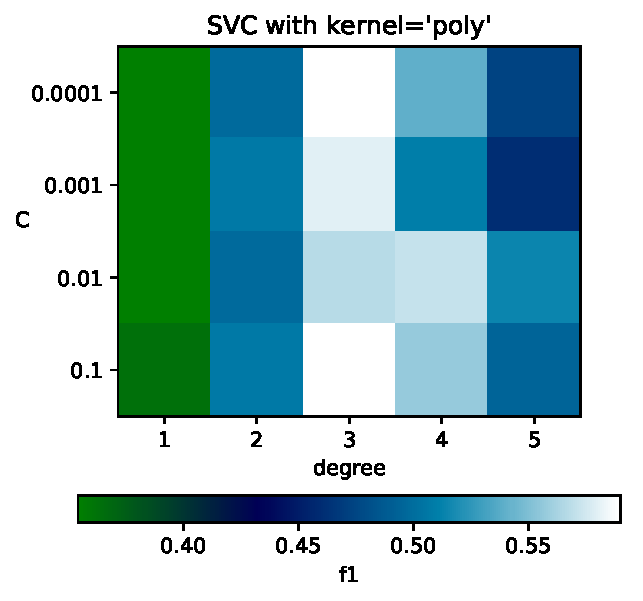
\includegraphics[width=.4\linewidth]{images/SVC_poly_degree.pdf}
	\caption{Rezultati SVC klasifikatora sa polinomijalnim kernelom (parametar \textit{gamma} je izostavljen sa slike zbog 2D prikaza)}
	\label{fig:svc-poly-degree}
\end{figure}

Sada kada znamo koji kerneli daju dobre ocene za naš problem potrebno je samo još detaljnije precizirati parametre \textit{C} i \textit{gamma} za obučavanje modela. Kada uporedimo ove rezultate na istoj skali, što možemo videti na slici \ref{fig:svc-results-best}, \textit{rbf} kernel pobeđuje.

\begin{figure}[h!]
	\centering
	\begin{subfigure}{.8\textwidth}
		%\centering
		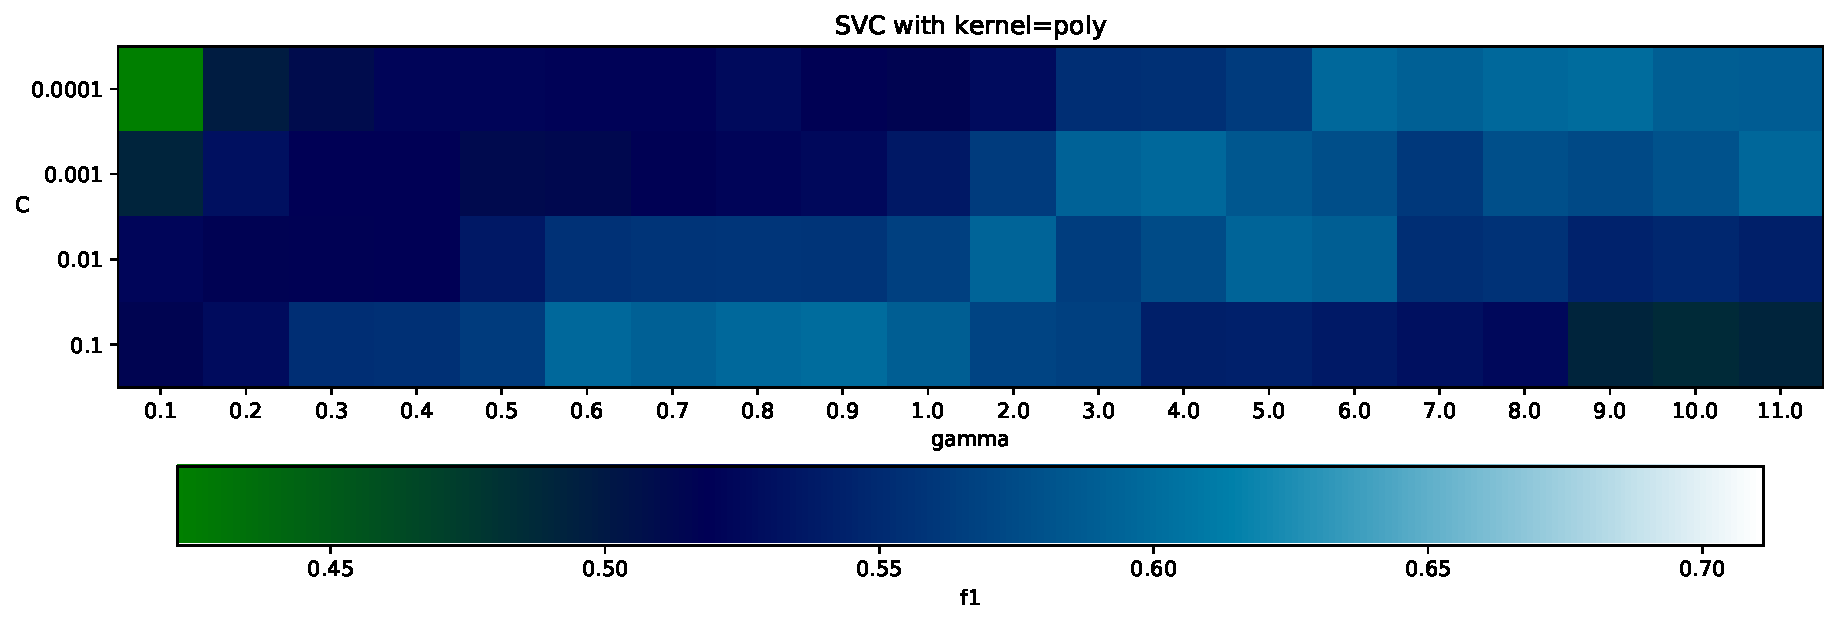
\includegraphics[width=1\linewidth]{images/SVC_kernel_fine_poly.pdf}
		\caption{Rezultati za polinomijanlni kernel}
		\label{fig:sub-best1}
	\end{subfigure} % or \hspace{5mm} or \hspace{0.3\textwidth}

	\begin{subfigure}{.6\textwidth}
		%\centering
		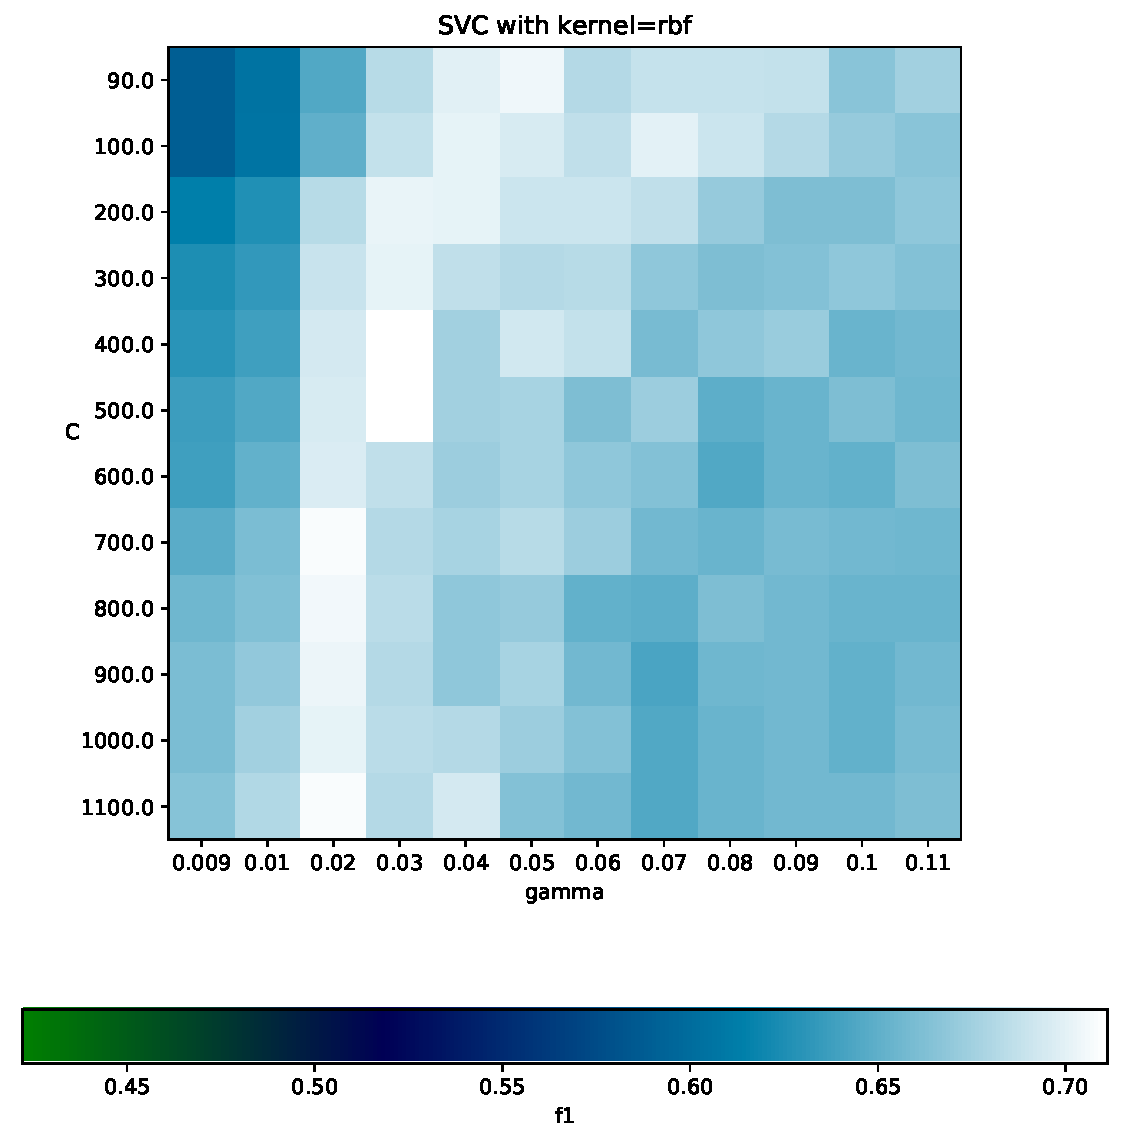
\includegraphics[width=1\linewidth]{images/SVC_kernel_fine_rbf.pdf}
		\caption{Rezultati za rbf kernel}
		\label{fig:sub-best2}
	\end{subfigure}
	\caption{Rezultati SVC klasifikatora sa preciznijim parametrima}
	\label{fig:svc-results-best}
\end{figure}

Kao konačnu ocenu ova dva kernela dajemo prosek rezultata 4-slojne unakrsne validacije (tabela \ref{tab:svc-final-results}), obučavajući oba modela sa parametrima koji su dali najbolju ocenu u prethodnom poređenju.

\begin{table}[h!]
	\centering
	\begin{tabular}{ |c|c|c|c|c| }
		\hline
		Kernel & F1 & Accuracy & Precision & Recall \\ 
		\hline
		%rbf & 0.650532227711313 & 0.9732850618511256 & 0.5518657305990604 & 0.7930881112211584 \\
		rbf & 0.651 & 0.973 & 0.552 & 0.793 \\
		\hline
		%poly & 0.61856412175831 & 0.9691302132537465 & 0.5051864846526862 & 0.7983911998826162  \\	
		poly & 0.619 & 0.969 & 0.506 & 0.798 \\
		\hline
	\end{tabular}
	\caption{Ocene odabranih klasifikatora}
	\label{tab:svc-final-results}
\end{table}

\newpage

\section{Moguća poboljšanja}

Jasno se uočava da je izbor atributa od ključnog značaja za uspešnu klasifikaciju ovog problema. Prilikom obučavanja modela korišćeno je 28 različitih atributa koji su predstavljeni numerički i daju informacije samo o jednoj slici. Svaka instanca se prilikom klasifikacije posmatra odvojeno od ostalih. 

Neki atributi kao što je broj slika istih dimenzija u dokumentu sa sobom nose neki širi kontekst, ali postavlja se pitanje da li je to dovoljno. Uvođenje atributa koji nose dodatne informacije o samom dokumentu bi mogle povećati ocenu modela, ali glavni problem je u odlučivanju korisnih atributa. Na primer, da li se u blizini slike nalazi dosta teksta može biti dobar indikator o tome da li ona pripada glavnom delu nekog članka. Međutim, problem definisanja ,,blizine'' jednog elementa drugom kao i pouzdano određivanje tog svojstva unutar HTML koda predstavlja problem, pogotovo kada uzmemo u obzir da ne postoji standardna tehnika za sastavljanje veb stranica kao i veliki broj različitih stilova.

Osim u slučaju linearnog kernela, tumačenje obučenog modela metodom potpornih vektora ne pruža jasne informacije o kvalitetu odabranih atributa. Nažalost, linearni kernel se pokazao kao lošija varijanta po tumačenje takvih koeficijenata ne mora biti pouzdano. Odbacivanje lošijih atributa može poboljšati performanse ali ispitivanje velikog broja mogućih kombinacija predstavlja dugotrajan proces koji ne mora nužno doneti i poboljšanja u oceni klasifikacije.

\section{Zaključak}
\label{sec:zakljucak}

Metod potpornih vektora se pokazao kao pouzdana i efikasna tehnika prilkom klasifikovanja relevantnih slika. Uz izbor atributa koji se mogu pouzdano izvući iz svake stranice kao i izbor odgovarajućih parametara dobija se visoka tačnost klasifikacije. 

\addcontentsline{toc}{section}{Literatura}
%\appendix
\bibliography{seminarski} 
\bibliographystyle{plain}

%\appendix
%\section{Dodatak}
%Ovde pišem dodatne stvari, ukoliko za time ima potrebe.


\end{document}
